\bookchapter{Chapter 49: Setting Up Your Development Environment — Android Studio and Your First Project}

\chapterintro{To do a good job, first sharpen your tools. In this chapter we set up the “kitchen”: install Android Studio, get the emulator running, create the first Android project of your life, then take the project structure apart until it makes sense. Once the environment is set up, you'll see your own code turn into a tappable button for the first time — a moment many people remember for the rest of their lives.}

\booksection{I. Installing Android Studio}

Android Studio is Google's official integrated development environment (IDE). It's free and a full all-in-one package: writing code, previewing UI, debugging, and packaging all happen inside it. Four steps to install:

\begin{enumerate}
  \item Open the official site developer.android.com/studio and download the latest stable version (as of August 2026, the release after Narwhal; Windows/Mac/Linux builds are all available);
  \item Run the installer and click "Next" all the way through — the setup wizard automatically includes the Android SDK and emulator components;
  \item On first launch, download the SDK components as prompted (the default selections are fine; it may take a few minutes and a few GB of space);
  \item When it's done you'll see the welcome screen — congratulations, the "kitchen" is set up.
\end{enumerate}

\begin{tcbwarn}{Note: Know the Hardware Requirements}
Android Studio is a memory hog: 16GB of RAM is recommended (8GB will run, but the emulator can lag), reserve at least 20GB of disk, and your CPU needs virtualization support (enable VT-x/AMD-V in the BIOS). If your computer really is old, use “real device debugging” instead of the emulator (covered in Section 4 of this chapter) — the experience is actually smoother.

\end{tcbwarn}

\booksection{II. Creating Your First Project}

On the welcome screen click New Project and pick the Empty Activity template (the cleanest beginner template), then fill in three things:

\begin{center}
\begin{tabularx}{\linewidth}{|X|X|X|}
\hline
\textbf{Setting} & \textbf{What to Enter} & \textbf{Notes} \tabularnewline
\hline
Name & My First App & The app's name, shown on the phone's home screen \tabularnewline
Package name & com.example.myfirstapp & A globally unique identifier; the convention is a reversed domain name — keep the default for now \tabularnewline
Minimum SDK & API 26(Android 8.0) & Minimum supported version; covers 95\%+ of devices \tabularnewline
\hline
\end{tabularx}
\end{center}

\begin{center}\small\color{gray}The three things to fill in when creating a project\end{center}

After you click Finish, Android Studio uses Gradle to automatically download dependencies and build the project (the first time takes a few minutes; every run after that is much faster). When the build finishes, you have a runnable app — even if it can only display one line: “Hello Android!”.

\begin{tcbinfo}{Tip: The Ins and Outs of Package Names}
The package name is like the app's “ID number” — it must be globally unique and can't be changed after publishing. For personal practice, com.example.xxx is fine; for a real product, switch to your own domain in reverse (like com.yourname.appname). Never publish with com.example — the store will reject it.

\end{tcbinfo}

\booksection{III. Running It: Emulator and Real Device}

The code is written — now you need a “phone” to run it on. You have two choices:

\booksubsection{The Emulator}

An emulator is a virtual Android phone inside your computer. In Android Studio, open Device Manager > Create Device, pick a device (the Pixel series is recommended) > choose a system image (one with Google APIs) > download > launch. Then click the green triangle Run in the toolbar, and a few seconds later your app appears on the “phone” screen.

\booksubsection{Real Device Debugging (More Recommended)}

A real phone is always the truest test environment — swipe feel, real network, real sensors; the emulator can't match any of it. Debugging on a real Android phone is simple:

\begin{enumerate}
  \item On the phone, open [Settings] > [About phone] and tap "Build number" 7 times in a row to unlock "Developer options";
  \item In [Developer options], turn on USB debugging;
  \item Connect the phone to the computer with a data cable and choose "Allow USB debugging" in the popup;
  \item Back in Android Studio, your phone appears in the device dropdown in the toolbar — click Run.
\end{enumerate}

\textbf{Watch Out: Don't Leave USB Debugging On}\par

USB debugging is like opening a “back door” to your phone for computers. When charging in public or connecting to a computer you don't trust, be sure to turn USB debugging off so no one can read your data through it. Turn it off after each development session — make it a habit.

\booksection{IV. Project Structure Explained: What Each File Does}

The file tree on the left can make your head spin the first time you open a project. Don't panic — in daily development, 90\% of your time is spent with just these few:

\begin{center}
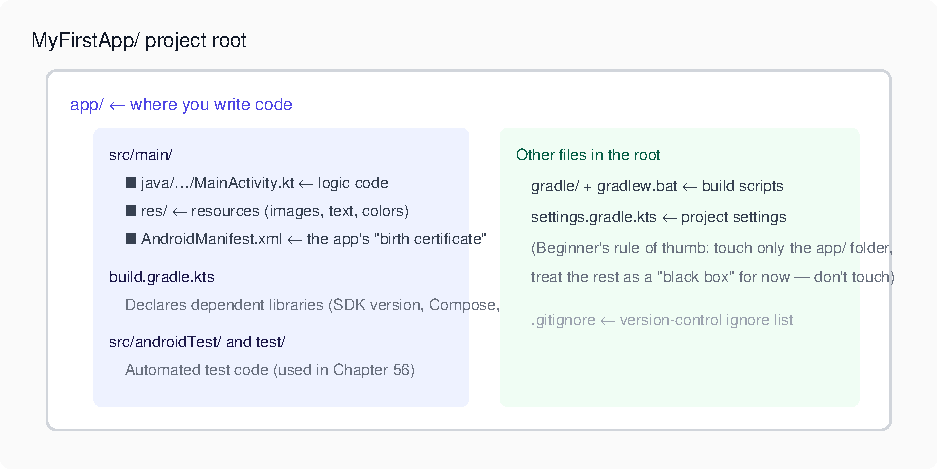
\includegraphics[width=0.92\linewidth]{figures/fig-di-si-shi-jiu-zhang-1}
\\[2pt]\small Figure 2: Project structure every beginner must know (the mantra: only touch the app/ folder)
\end{center}

\begin{itemize}
  \item MainActivity.kt: the app's "front door." When a user taps the icon, this is the first thing to wake up. In the current template it's responsible for displaying "Hello Android!".
  \item AndroidManifest.xml: the app's "household registry" — it declares what this app is called, which icon it uses, which screens it has, and which permissions it needs (camera, location, etc.).
  \item The res/ folder: the resource warehouse, storing images, icons, strings, and colors. Keeping text in resource files instead of hard-coding it into code is a good habit in Android development (it makes switching languages or themes easy).
  \item build.gradle.kts: the build recipe — it declares the minimum supported version and which libraries to depend on (like Compose).
\end{itemize}

\booksection{V. A First Try: Change “Hello” to Your Name}

Open MainActivity.kt and you'll see the code the Compose template generated. Find the line Text(“Hello Android!”) and replace the text inside the quotes with your name, e.g. Text(“Hi, Zhang San! This is my first app”), then press Ctrl+R (Cmd+R on Mac) to run again. A few seconds later, your name appears on the emulator.

\begin{lstlisting}[language=Kotlin]
setContent {
    MyFirstAppTheme {
        Surface(modifier = Modifier.fillMaxSize()) {
            // v change this to your own text
            Text("Hello, Alex! This is my first app")
        }
    }
}
\end{lstlisting}

Congratulations — you've just completed a full “edit code compile install run” cycle. This cycle is your daily development routine from now on. Strike while the iron is hot and change something else: make the font bigger, try another color — the next chapter shows where these “magic powers” come from.

\booksection{VI. First Aid for Common Errors: The Beginner's “ER” for Your First Two Weeks}

During environment setup and your first build, you'll most likely hit the three errors below. Don't panic — all of them have antidotes:

\begin{center}
\begin{tabularx}{\linewidth}{|X|X|X|}
\hline
\textbf{Error} & \textbf{Common Cause} & \textbf{Fix} \tabularnewline
\hline
Gradle sync failed / slow dependency downloads & Poor network access to the repositories & Configure a mirror repository for Gradle (Alibaba Cloud / Tencent Cloud Maven mirrors); search online for "gradle China mirror" and follow the instructions \tabularnewline
Missing SDK components & The SDK download was skipped during installation & Settings > SDK Manager: install the missing platforms and tools \tabularnewline
Emulator fails to start / black screen & Virtualization not enabled, or a corrupted image & Enable VT-x/AMD-V in the BIOS; delete and recreate the emulator; or just debug on a real device \tabularnewline
\hline
\end{tabularx}
\end{center}

\begin{center}\small\color{gray}First-Aid Table for Beginner Environment Errors\end{center}

\begin{tcbinfo}{Tip: How to Search Error Messages}
The first line of an error message is the most valuable — copy it verbatim into a search engine and add the keyword “android studio”. Don't search vague questions like “why can't I set up my environment”; search specific errors like “Gradle sync failed: Could not resolve com.android.tools.build”. Precise questions get precise answers.

\end{tcbinfo}

\begin{tcbpractice}{Hands-On: Complete Your "Developer Ritual" Checklist}
(1) Install Android Studio and get the emulator running; (2) run your app on a real phone once and take a screenshot to keep; (3) change the Hello text to your name; (4) zip up the project as a backup. Once these four steps are done, you can announce to your friends: I'm an Android developer now (screenshot as proof).

\end{tcbpractice}

\begin{tcbsummary}{Chapter Summary}
\begin{itemize}
  \item Android Studio = the official free IDE; recommended 16GB RAM + 20GB disk + virtualization enabled
  \item Three essentials for a new project: name, package name (globally unique, never publish com.example), minimum SDK (API 26 or higher)
  \item Two ways to run: the emulator (a virtual phone on your computer) and a real device (enable USB debugging, remember to turn it off after)
  \item Project mantra: only touch the app/ folder — MainActivity.kt is the front door, the Manifest is the household registry, res/ is the resource warehouse
  \item The developer's daily loop = edit code Run check the result, over and over
\end{itemize}

\end{tcbsummary}
